% -*- fill-column: 110 -*-
\documentclass[12pt]{article}
\usepackage[margin=1in]{geometry}
\usepackage{hyperref}
\usepackage{graphicx}
\usepackage{amsmath}
\usepackage{amsfonts}
\usepackage{amssymb}
\usepackage{amsthm}
\usepackage[margin=1in]{geometry}
% \usepackage{apacite}
\usepackage{color}
%\usepackage{sagetex}
\usepackage{fancyhdr}
\usepackage{setspace}
\pagestyle{fancy}
\lhead{\footnotesize Outline for IDS499 final project}
\rhead{\footnotesize October 12 2013 -- IDS499 -- Shae Erisson}

\author{Shae Matijs Erisson\\Interdisciplinary Studies Department\\University of North Alabama}
\title{Statistical Learning for User-Specific Webpage Recommendations}
\begin{document}
\date{October 12 2013}
\maketitle{}
\pagebreak{}
%\section*{Statistical Learning for User-Specific Webpage Recommendations}

\begin{abstract}
  This paper and its associated software will explore the use of statistical learning to find previously
  unknown webpages of interest to the user of the software.

  We focus on the use of support vector machines to do supervised learning that results in efficient
  categorization of web pages into interesting or uninteresting.

  We also present a prototype web-based tool that allows the user to train their own nonlinear statistical
  classifier to find web pages specific to a particular subject of interest.
\end{abstract}
\pagebreak{}
\section{Introduction}
Can statistical classifiers be used to expand rather than filter knowledge?

Much time is spent trying to find relevant web sites when doing research for any number of tasks. While those
helpful websites exist for almost any subject, it can be difficult to find which website is best for a
particular topic.

While searching Google can be fun, sometimes too much time is spent trying to find relevant information, or
irrelevant search results become distrating from the actual

Up to now statistical classifiers have primarily been used to automatically categorize items based on a user's
feedback. In fact, this is how most spam filters function. Since each person will consider different messages
to be useful content, and so each person must give their own feedback to the filter.

Services such as Netflix and Amazon use similar software to suggest movies or books according to which movies
or books the user has already enjoyed.

The research problem we address here is whether this can be generalized to recommending webpages to the user
according to which webpages they've found relevant in the past.
\section{Justification for the Study}
Statistical learning has been used to filter spam for decades. In that specific case, the filtering works by
increasing or decreasing the score of a particular message by summing the score of each word in the contents.
These statistics are trained for each user, so the word mortgage might have a positive score for a bank
employee, where mortgage would have a negative score for most people.

This research project proposes to use support vector machines to find new results rather than filter out
existing content. The project consists of both prototype software and a report describing the results.

% The software will watch the user browsing the web and uses that input to build Bayesian statistics for later
% searching for new documents of interest.
\section{Statistical Classifiers}
% This section will give an overview of statistical classifiers. 

The goal of a classifier is to sort inputs into different categories based on features of those inputs. The
most familiar examples would be book recommendations from Amazon and movie recommendations from Netflix. Those
recommendations are done with software that has determined important features of all the books and movies
available, and has some way to figure out which books or movies are similar to which other books or
movies. \cite{michie1994machine}

Statistical classifiers are divided into two major types, linear classifiers and 
\subsection{Linear Classifiers}
Linear classifiers are called linear because, given a set of points drawn in a two dimensional space, the
classifier finds a line that divides the space into two halves where one side of the line is one category, and
the other side of the line is the other.\\
% center this? XXX
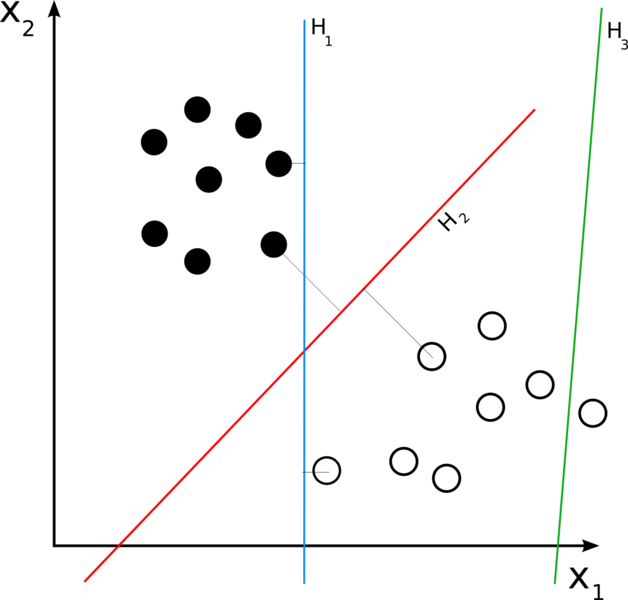
\includegraphics[scale=.4,natwidth=628,natheight=600]{svm_separating_hyperplanes.png}\\
This section will describe the simplest instance of linear statistical classifiers, Naive Bayesian
Classifiers. \cite{kononenko1991semi}
\subsection{Support Vector Machines}
This section will describe the nonlinear statistical classifier that will be used in this software
prototype. \cite{hearst1998support}
\subsection{Others}
This section will cover the range of other statistical classifiers in less detail.
\section{Common uses of Statistical Classifiers}
\subsection{Spam Filters}
This will describe how statistical classifiers are used in spam filters. \cite{androutsopoulos2000evaluation}
\subsection{Natural Language Guessing}
This will describe how statistical classifiers are used in guessing \cite{martins2005language}
the natural language used in a document.
\subsection{Topic Categorization}
This will describe how statistical classifiers are used to automatically choose a category for text
content. \cite{pang2002thumbs}
\subsection{Malware Detection}
This will describe how statistical classifiers are used to detect malware on computers.\\ \cite{perdisci2008mcboost}
\subsection{Movie and Book Recommendations}
This will describe how statistical classifiers are used to recommend movies \cite{basu1998recommendation} and
books \cite{linden2003amazon} based on the movies or books previously enjoyed by a user.
\section{Existing Tools}
\subsection{Google Prediction API}
This will describe the Google Prediction API. \cite{GooglePrediction:2013:Online}
\subsection{NLTK}
This will describe the Natural Language Toolkit library. \cite{NLTK:2013:Online}
\section{Proposed Software}
\subsection{Transparent Proxy}
This will describe the use of a transparent proxy to capture the text
of the webpages that the user views.
\subsection{Statistical Classifier}
This will describe populating the statistical classifier from the text
of the viewed webpages.
\subsection{Predictive Model}
This will describe how the classifier can be used to find new and
interesting results for the user.
\subsection{User Interface}
This will describe the web based front end for the system, including
how the user will train the software.
\section{Possible Uses}
\subsection{Personal and Corporate Research}
Once trained for a particular subject, this software could run in the
background looking for new results, much like a news feed.
\subsection{Research Paper Analysis}
If a user has a large collection of research papers and would like to
pick out which papers may be relevant, the software could discover this.
\section{Future Directions}
\subsection{Overfocus Prevention}
One of the problems with statistical classifiers is that they can be
over trained and end up limiting the results, thus missing results the
user may not yet know they wish to see.
This section will describe possible strategies for resolving that
issue.
\subsection{Multiuser}
One of the best ways to inject new results into an over trained system
may be to import the best results from other users who have agreed to
share their results.
\subsection{Ease of Use}
The current design for the software requires the user to have a
transparent proxy configured in the web browser.
This section will consider options such as a Firefox Extension or a
Chrome Plugin so that setup will only require clicking.
\pagebreak{}
\bibliographystyle{apalike} 
\bibliography{outline}
\end{document}

% LocalWords: LocalWords differentiable
 

%%% Local Variables: 
%%% mode: latex
%%% TeX-master: t
%%% End: 
